\documentclass[a4paper,11pt,reqno,french,dvipsnames,table]{article}

% Les paramètres dvipsnames passés sont passés à xcolor, déjà appelé par TikZ.
% Pareil, le param "table" est pour le param table passé à xcolor pour la coloration de cellules.

\usepackage{../utilities}

\usepackage{graphicx}

\usepackage{transparent} % Pour les trous

\usepackage{tabularx}                                               % Pour tableaux mais avec + de possibilités (tabular de base + mais tabularx offre possibilités ++)


\captionsetup[figure]{labelformat=empty} % Pour ne pas afficher le "Figure # : " dans les captions.


\definecolor{boxTitle}{HTML}{fff79a}
\definecolor{boxBackground}{HTML}{fffce0}
\definecolor{boxFrame}{HTML}{f1e2b8}

\definecolor{rougeClair}{HTML}{ffc7c7}
\definecolor{rougeFonce}{HTML}{c81111}

\definecolor{bleuClair}{HTML}{c1e7ff}
\definecolor{bleuFonce}{HTML}{1166c8}

\definecolor{vertClair}{HTML}{c3ffc1}
\definecolor{vertFonce}{HTML}{11c728}

\definecolor{grisClair}{HTML}{c4c4c4}

\definecolor{clrgrillemajeure}{HTML}{696969}
\definecolor{clrgrillemineure}{HTML}{9c9c9c}

\definecolor{colonnegauchetableau}{HTML}{dddddd}
\definecolor{orangeAttentionClair}{HTML}{ff8b61}

% Pour la police manuscrite par exemple pour citations de vieux textes historiques.
\newfontfamily\policemanuscrite{QTBlackForest}

% Pour du texte en grec (e.g. mot d'origine grecque).
\newfontfamily\policegrecque{Cardo}
\newcommand{\grec}[1]{\bgroup\policegrecque{#1}\egroup}



\newcommand{\partieDeCours}[1] {
	\vspace{5pt}
	\newpage
	\begin{center}
		\begin{tikzpicture}
			
			\node[black] (partname) at (0,0) {\Large \textbf{\textrm{#1}}};
			
			\draw[black,thick] (partname.north west) + (-1,0.4) -- ($(partname.north east)+(1,0.4)$);
			\draw[black,thick] (partname.south west) + (-1,-0.4) -- ($(partname.south east)+(1,-0.4)$);
			
		\end{tikzpicture}
	\end{center}
	\vspace{5pt}
}

% Le tag 'breakable' pour les boîtes n'est pas présent car ma tutrice n'aime pas voire les boîtes cassées et renvoyées à la page suivante. J'aime bien perso et l'activerais quand j'aurai le contrôle total. 

% pre scriptum : la compil est longue en partie à cause des saloperies d'icônes bs-truc qui sont converties du format MS à PDF, méthode à changer. -> C bo mais c long.

\tcbset{boite def/.style={
		%breakable,
		enhanced,
		fonttitle=\bfseries,
		colback=white,
		sharp corners,
		colbacktitle=rougeClair,
		colframe=rougeFonce,
		coltitle=black,
		attach boxed title to top left={xshift=0.3cm,yshift*=-\tcboxedtitleheight/2},
		boxed title style={
			before upper=\hspace*{0.5cm}, % reserve space for the image
			overlay={
			 \node at ([xshift=0.5cm]frame.west)
				 {\small \emoji{brick}};
			}
		}
	}
}

\tcbset{boite propo/.style={
		%breakable,
		enhanced,
		fonttitle=\bfseries,
		colback=white,
		colbacktitle=bleuClair,
		colframe=bleuFonce,
		coltitle=black,
		attach boxed title to top left={xshift=0.3cm,yshift*=-\tcboxedtitleheight/2},
		boxed title style={
			before upper=\hspace*{0.5cm}, % reserve space for the image
			overlay={
			 \node at ([xshift=0.5cm]frame.west)
				 {\small \emoji{wrench}};
			}
		}
	}
}

\tcbset{boite exe/.style={
		%breakable,
		blanker,
		left=5mm,
		top=5mm,
		bottom=5mm,
		borderline west={1mm}{0pt}{vertFonce},
		enhanced, fonttitle=\bfseries,
		colback=white,
		colbacktitle=vertClair,
		colframe=vertFonce,
		coltitle=black,
		attach boxed title to top left={xshift=0.3cm,yshift*=-\tcboxedtitleheight/2},
		boxed title style={
			before upper=\hspace*{0.5cm}, % reserve space for the image
			overlay={
			 \node at ([xshift=0.5cm]frame.west)
				 {\small \emoji{pencil}};
			}
		}
	}
}

\tcbset{boite cult/.style={
		%breakable,
		enhanced,
		fonttitle=\bfseries,
		colback=white,
		coltitle=black,
		colbacktitle=grisClair,
		frame empty,
		borderline={0.5mm}{0mm}{black,dashed},
		attach boxed title to top left={xshift=0.3cm,yshift*=-\tcboxedtitleheight/2},
		boxed title style={
			before upper=\hspace*{0.5cm}, % reserve space for the image
			overlay={
			 \node at ([xshift=0.5cm]frame.west)
				 {\small \emoji{musical-note}};
			}
		}
	}
}

\newtcolorbox{boiteDefinition}[1][]{boite def, #1}
\newtcolorbox{boiteProposition}[1][]{boite propo, #1}
\newtcolorbox{boiteExemple}[1][]{boite exe, #1}
\newtcolorbox{boiteCulture}[1][]{boite cult, #1}

% Pour remonter un peu le pied de page (genre numérotation des pages) car trop bas à cause des marges faibles.
\setlength{\footskip}{-0.4cm}

% Paramétrage de la taille de la feuille.
\geometry{
	a4paper,
	total={170mm,257mm},
	left=20mm,
	top=10mm,
	bottom=10mm
}

\pgfplotsset{
	every tick label/.append style={font=\boldmath}
}

\tikzstyle{every node}=[font=\Large]


% Pour cacher le texte
\newcommand{\trou}[1]{\textcolor{white}{#1}}
% Pour révéler le texte
%\newcommand{\trou}[1]{#1}


\begin{document}

\vspace*{\fill}

\begin{center}
	
	\Huge
	
	\textbf{Limites et continuité de fonctions}
	
\end{center}

\vspace*{\fill}

\begin{center}
	
	\parbox{0.7\textwidth}{
		\begin{center}
			\policemanuscrite
			\Large
			\textit{Le terme d'une progression est la fin des séries, à laquelle aucune progression ne peut aboutir, s'il nous est permis de la poursuivre à l'infini; mais à laquelle il est possible d'accéder d'aussi près que de n'importe quel intervalle donné.}
		\end{center}
	}
	
\end{center}

\begin{flushright}
	\textit{OPUS GEOMETRICUM} (1647), Gréoire de Saint-Vincent.
\end{flushright}

\vspace*{\fill}

\begin{figure}[H]
	
	\centering
	
	\begin{minipage}[b]{.3\pagewidth}
		\centering
		\begin{tikzpicture}
			\begin{axis}[
				grid = major,
				axis line style = very thick,
				grid style={line width=1pt, draw=gray!50},
				axis equal image,
				xmin=-2,xmax=12,
				ymin=-2,ymax=8,
				xtick = {-2,...,12},
				ytick = {-2,...,8},
				axis lines=middle,
				axis line style={-Latex},
				ticks=none
			]
			
				% Asymptote horizontale
				\draw[color=red, thick] (axis cs:-2,3.5) -- (axis cs:12,3.5);
				
				\addplot[
					domain=0:12,
					samples=13,
					color=blue,
					only marks
					] {3.5 + 30*sin(180*(x + 1) / pi) / ((x+3)^2)};
			
			\end{axis}
		\end{tikzpicture}
	\end{minipage}
	\hspace{1cm}
	\begin{minipage}[b]{.3\pagewidth}
		\centering
		\begin{tikzpicture}
			\begin{axis}[
				grid = major,
				axis line style = very thick,
				grid style={line width=1pt, draw=gray!50},
				axis equal image,
				xmin=-2,xmax=12,
				ymin=-2,ymax=8,
				xtick = {-2,...,12},
				ytick = {-2,...,8},
				axis lines=middle,
				axis line style={-Latex},
				ticks=none
			]
				
				% Asymptote horizontale
				\draw[color=red, thick] (axis cs:-2,3.5) -- (axis cs:12,3.5);
				
				\addplot[
					domain=-2:12,
					samples=100,
					color=blue,
					thick
					] {3.5 + 30*sin(180*(x + 1) / pi) / ((x+3)^2)};
				
				% Le 'cs' de 'axis cs' signifie 'coordinates system' pour se référer au système de coordonnées du graphique généré par pgfplots, car le \draw est une commande TikZ ne se basant par sur les coordonnées des axes de PGFPlots.
				
			\end{axis}
		\end{tikzpicture}
	\end{minipage}
	
	\caption{\textit{Deux concepts similaires : limite de suite et limite de fonction.}}
	
\end{figure}


\vspace*{\fill}

% Pas de notation de n° de page pour la page de garde
\thispagestyle{empty}








\partieDeCours{Partie 1 : Limites en $+ \infty$ et en $- \infty$}

\pagenumbering{arabic}

% Comment instancier f intelligement sans rentrer dans un détail trop technique "Soit f une fonction définie au voisinage de \pm l'infini" ? Tant que pas réfléchir dessus, préfère passer outre (comme fait dans le Barbazo).

\begin{boiteDefinition}[title={Définition : limite finie}]
	
	\begin{figure}[H]
		\centering
		\begin{minipage}{.3\linewidth}
			\centering
			\begin{tikzpicture}
				\centering
				\begin{axis}[
					grid = both,
					axis line style = very thick,
					minor grid style={line width=0.4pt, draw=black!30},
					major grid style={line width=0.5pt, draw=black!60},
					axis equal image,
					xmin=-3,xmax=6,
					ymin=-2,ymax=5,
					xtick = {-3,-2,...,6},
					ytick = {-2,-1,...,5},
					xticklabels={},
					yticklabels={},
					extra y ticks = {3},
					extra y tick style={tick label style={anchor=south east}},
					minor x tick num=1,
					minor y tick num=1,
					axis lines=middle,
					axis line style={-Latex},
					xlabel=$x$,
					xlabel style = {at={(axis description cs:1,0.260714286)},anchor=north east}
				]
					
					% Graphe de la fonction
					\addplot[
						domain=-3:6,
						samples=200,
						color=blue,
						thick] {3 - 1 / (x+3.5)};
					
					% Asymptote horizontale
					\draw[color=red, thick] (axis cs:-3,3) -- (axis cs:6,3);
					
					
					\node [color=blue,thick] at (axis cs:-2,1.5) {$\mathscr C_f$};
					\node [color=red,thick] at (axis cs:-2,3.5) {$y = 3$};
					
				\end{axis}
			\end{tikzpicture}
		\end{minipage}
		\hspace{2.4cm}
		\begin{minipage}[c]{.5\linewidth}
			On dit que la fonction $f$ admet pour limite un réel $l$ lorsque $x$ tend vers $+\infty$ si $f(x)$ se rapproche autant de $l$ que l'on veut dès que $x$ est assez grand.
			
			On note \trou{$\limite{x \to \infty} f(x) = l$.}
			
			\vspace{10pt}
			
			On définit la limite de manière similaire en $- \infty$.
			
			On note \trou{$\limite{x \to -\infty} f(x) = l$.}
		\end{minipage}
		
	\end{figure}
	
	Ici, \trou{\underline{il semblerait}} que $\limite{x \to +\infty} = 3$ : $f(x)$ se rapproche de $3$ autant que possible quand $x$ est assez grand.

\end{boiteDefinition}

\begin{boiteExemple}[title={Exemples}]
	\begin{figure}[H]
		\centering
		\begin{minipage}{.3\linewidth}
			\centering
			\begin{tikzpicture}
				\centering
				\begin{axis}[
					grid = both,
					axis line style = very thick,
					minor grid style={line width=0.4pt, draw=black!30},
					major grid style={line width=0.5pt, draw=black!60},
					axis equal image,
					xmin=-9,xmax=9,
					ymin=-7,ymax=7,
					xtick = {-10,-5,...,10},
					ytick = {-10,-5,...,10},
					xmajorticks=true,
					minor x tick num=4,
					minor y tick num=4,
					axis lines=middle,
					axis line style={-Latex},
					xlabel=$x$,
					xlabel style = {at={(axis description cs:1,0.475)},anchor=north east}
				]
					
					\addplot[
						domain=-9:9,
						samples=200,
						color=blue,
						thick] {7*e^x / (1 + e^x) - 4 + 5 / (1 + x^2) * sin(180 * x / pi * 2)};
					
					\node [color=blue,thick] at (axis cs:6,4) {$\mathscr C_f$};
					
				\end{axis}
			\end{tikzpicture}
		\end{minipage}
		\hspace{2.4cm}
		\begin{minipage}[c]{.5\linewidth}
			On a tracé ci-contre la courbe représentative de la fonction $f$.
			
			Graphiquement, on peut \underline{conjecturer} que :
			\begin{itemize}
				\item \trou{$\limite{x \to +\infty} f(x) = 3$.}
				\item \trou{$\limite{x \to -\infty} f(x) = -4$.}
			\end{itemize}
		\end{minipage}
	\end{figure}
	
	\noindent\makebox[\textwidth]{\rule{\textwidth}{1pt}}
	
	Voici un exemple de fonction qui n'admet pas de limite en $+\infty$, la fonction \trou{cosinus} :
	
	\begin{figure}[H]
		\centering
		\begin{tikzpicture}[scale=1.5]
			\begin{axis}[
				grid = both,
				axis line style = very thick,
				minor grid style={line width=0.4pt, draw=black!30},
				major grid style={line width=0.5pt, draw=black!60},
				axis equal image,
				xmin=-10,xmax=10,
				ymin=-3,ymax=3,
				xtick = {-10,-5,...,10},
				ytick = {-2,0,2},
				xticklabels={},
				yticklabels={},
				minor x tick num=4,
				minor y tick num=1,
				axis lines=middle,
				axis line style={-Latex},
				xlabel=$x$,
				xlabel style = {at={(axis description cs:1,0.65)},anchor=south east}
			]
				
				% Graphe de la fonction
				\addplot[
					domain=-10:10,
					samples=200,
					color=blue,
					thick] {cos(180 * x / pi)};
				
			\end{axis}
		\end{tikzpicture}
	\end{figure}
	
\end{boiteExemple}

\begin{boiteProposition}[title={Limites de fonctions de référence (admises)}]
	
	\begin{figure}[H]
		\centering
		\begin{minipage}[c]{.3\linewidth}
			\centering
			\begin{tikzpicture}
				\centering
				\begin{axis}[
					grid = major,
					axis line style = very thick,
					grid style={line width=0.5pt, draw=black!60},
					axis equal image,
					xmin=-6,xmax=6,
					ymin=-6,ymax=6,
					xtick = {-6,...,6},
					ytick = {-6,...,6},
					axis lines=middle,
					axis line style={-Latex},
					xticklabels={},
					yticklabels={},
					extra x ticks={1},
					extra y ticks={1},
					xlabel=$x$,
					xlabel style = {at={(axis description cs:1,0.475)},anchor=north east}
				]
					
					\addplot[
						domain=-6:1.8,
						samples=100,
						color=blue,
						thick] {e^(x)};
					
					\node [color=blue,thick] at (axis cs:3.5,3.5) {$x \mapsto \trou{e^x}$};
					
					% Les deux comp. co. du graphe de l'hyperb. canon.
					\addplot[
						domain=-6:-0.1,
						samples=100,
						color=Green,
						thick] {1 / x};
					\addplot[
						domain=0.1:6,
						samples=100,
						color=Green,
						thick] {1 / x};
					
					\node [color=Green,thick] at (axis cs:4,1.5) {$x \mapsto \trou{\frac{1}{x}}$};
					
				\end{axis}
			\end{tikzpicture}
		\end{minipage}
		\hspace{1cm}
		\begin{minipage}[c]{.3\linewidth}
			\centering
			\Large
			$\limite{x \to +\infty} \frac{1}{x} = \trou{0}$ \\
			\vspace{30pt}
			$\limite{x \to -\infty} \frac{1}{x} = \trou{0}$ \\
			\vspace{30pt}
			$\limite{x \to -\infty} e^x         = \trou{0}$
		\end{minipage}
	\end{figure}
\end{boiteProposition}


\begin{boiteDefinition}[title={Définition : asymptote horizontale}]
	
	La droite d'équation $y=l$ est dite une \trou{\underline{asymptote horizontale}} à la \trou{\underline{courbe représentative}} de $f$ :
	\begin{itemize}
		\item en $+\infty$ si \trou{$\limite{x \to \infty} f(x) = l$;}
		\item en $-\infty$ si \trou{$\limite{x \to -\infty} f(x) = l$.}
	\end{itemize}
	
\end{boiteDefinition}


\begin{boiteExemple}[title={Exemple}]
	Dans l'exemple de la page précédente, on peut conjecturer deux asymptotes au graphe \textcolor{blue}{$\mathscr C_f$} de $f$ :
	\begin{itemize}
		\item La droite d'équation \trou{$y=3$} en \trou{$+\infty$.}
		\item La droite d'équation \trou{$y=-4$} en \trou{$-\infty$.}
	\end{itemize}
	
	Pour utiliser une limite de référence : la courbe représentative de la fonction exponentielle admet la droite d'équation \trou{$y=0$} comme asymptote horizontale en \trou{$+\infty$.}
	
\end{boiteExemple}

	
\begin{boiteCulture}[title={Mot asymptote}]
Le mot "asymptote" vient du grec \grec{ἀσύμπτωτος} (asumptōtos) :
signifiant « qui ne coïncide pas ». Ce mot fut introduit par le mathématicien Apollonios de Perga (c.a. 240 avant J.C.) au moment où il étudiait les intersections de plans et de cônes (appellées \textit{coniques}).
\end{boiteCulture}




\begin{boiteDefinition}[title={Définition : limite infinie}]
	
	On dit que $f$ admet pour limite $+\infty$ lorsque $x$ tend vers $+\infty$ si $f(x)$ prend des valeurs de plus en plus grandes pour $x$ suffisament grand.
	
	On note \trou{$\limite{x \to +\infty} f(x) = +\infty$.}
	
	Si $f(x)$ prend des valeurs de plus en plus « basses » pour $x$ suffisament grand alors la limite en $+\infty$ de la fonction $f$ est $-\infty$.
	
	On note \trou{$\limite{x \to +\infty} f(x) = -\infty$.}
	
	\vspace{10pt}
	
	On définit de manière similaire les écritures \trou{$\limite{x \to -\infty} f(x) = +\infty$ et $\limite{x \to -\infty} f(x) = -\infty$.}
	
\end{boiteDefinition}

% Fait office d'illustration / exemple
\begin{boiteProposition}[title={Limites de fonctions de référence (admises)}]
	
	\begin{figure}[H]
		
		\centering
		
		\begin{minipage}[b]{.3\pagewidth}
			\centering
			\begin{tikzpicture}
				\begin{axis}[
					grid = major,
					axis line style = very thick,
					grid style={line width=0.5pt, draw=black!60},
					axis equal image,
					xmin=-5,xmax=5,
					ymin=-1,ymax=7,
					xtick = {-5,...,5},
					ytick = {-1,...,7},
					axis lines=middle,
					axis line style={-Latex},
					xticklabels={},
					yticklabels={},
					extra x ticks={1},
					extra y ticks={1},
					xlabel=$x$,
					xlabel style = {at={(axis description cs:1,0.025)}}
				]
					
					\addplot[
						domain=-5:5,
						samples=100,
						color=blue,
						thick] {x ^2};
					
					\node [color=blue,thick] at (axis cs:3,2.75) {$x \mapsto \trou{x^2}$};
					
				\end{axis}
			\end{tikzpicture}
		\end{minipage}
		\hspace{1cm}
		\begin{minipage}[b]{.3\pagewidth}
			\centering
			\begin{tikzpicture}
				\begin{axis}[
					grid = major,
					axis line style = very thick,
					grid style={line width=0.5pt, draw=black!60},
					xmin=-3,xmax=3,
					ymin=-5,ymax=5,
					xtick = {-3,...,3},
					ytick = {-5,...,5},
					axis lines=middle,
					axis line style={-Latex},
					xticklabels={},
					yticklabels={},
					extra x ticks={1},
					extra y ticks={1},
					xlabel=$x$,
					xlabel style = {at={(axis description cs:1,0.475)},anchor=north east}
				]
					
					\addplot[
						domain=-3:3,
						samples=100,
						color=blue,
						thick] {x ^3};
					
					\node [color=blue,thick] at (axis cs:-2,-1.5) {$x \mapsto \trou{x^3}$};
					
				\end{axis}
			\end{tikzpicture}
		\end{minipage}
		
		\centering
		\begin{minipage}[b]{.3\pagewidth}
			\centering
			\begin{tikzpicture}
				\begin{axis}[
					grid = major,
					axis line style = very thick,
					grid style={line width=0.5pt, draw=black!60},
					axis equal image,
					xmin=-6,xmax=3,
					ymin=-1,ymax=7,
					xtick = {-6,...,3},
					ytick = {-1,...,7},
					axis lines=middle,
					axis line style={-Latex},
					xticklabels={},
					yticklabels={},
					extra x ticks={1},
					extra y ticks={1},
					xlabel=$x$,
					xlabel style = {at={(axis description cs:1,0.025)}}
				]
					
					\addplot[
						domain=-6:3,
						samples=100,
						color=blue,
						thick] {e^(x)};
					
					\node [color=blue,thick] at (axis cs:-2,1.5) {$x \mapsto \trou{e^x}$};
					
				\end{axis}
			\end{tikzpicture}
		\end{minipage}
		\hspace{1cm}
		\begin{minipage}[b]{.3\pagewidth}
			\centering
			\begin{tikzpicture}
				\begin{axis}[
					grid = major,
					axis line style = very thick,
					grid style={line width=0.5pt, draw=black!60},
					xmin=-0.2,xmax=8,
					ymin=-0.2,ymax=4,
					xtick = {-1,...,8},
					ytick = {-1,...,4},
					axis lines=middle,
					axis line style={-Latex},
					xticklabels={},
					yticklabels={},
					extra x ticks={1},
					extra y ticks={1},
					xlabel=$x$,
					xlabel style = {at={(axis description cs:1,0.075)}}
				]
					
					\addplot[
						domain=0:8,
						samples=100,
						color=blue,
						thick] {sqrt(x)};
					
					\node [color=blue,thick] at (axis cs:2,3) {$x \mapsto \trou{\sqrt x}$};
					
				\end{axis}
			\end{tikzpicture}
		\end{minipage}
		{
			\Large
			\begin{align*}
				\limite{x \to +\infty} x^2 &= \trou{+\infty}   &     \limite{x \to -\infty} x^3 &= \trou{+\infty}   & \limite{x \to +\infty} e^x &= \trou{+\infty}   &  \limite{x \to +\infty} \sqrt x &= \trou{+\infty}    \\
				\limite{x \to -\infty} x^2 &= \trou{+\infty}   &     \limite{x \to -\infty} x^3 &= \trou{-\infty}   &  &
			\end{align*}
		}
	\end{figure}
\end{boiteProposition}

Compétences travaillées en exercices
\begin{itemize}
	\item Conjecturer des limites graphiquement sur schéma (donné ou sur la calculatrice).
	\item Conjecturer des limites à l'aide d'une expression sur la calculatrice.
\end{itemize}



\partieDeCours{Partie 2 : Limites en un réel $a$}


\begin{boiteDefinition}[title={Définition : limite infinie}]
	Soit $f$ une fonction définie sur un intervalle $I$. Soit $a$ un nombre réel.
	
	\begin{figure}[H]
		\centering
		\begin{minipage}{.3\linewidth}
			\centering
			\begin{tikzpicture}
				\centering
				\begin{axis}[
					grid = major,
					axis line style = very thick,
					minor grid style={line width=0.4pt, draw=black!30},
					major grid style={line width=0.5pt, draw=black!60},
					axis equal image,
					xmin=-7,xmax=7,
					ymin=-3,ymax=5,
					xtick = {-8,-6,...,8},
					ytick = {-4,-2,...,6},
					axis lines=middle,
					axis line style={-Latex},
					xticklabels={},
					yticklabels={},
					extra x ticks = {2},
					extra y ticks = {2},
					xlabel=$x$,
					xlabel style = {at={(axis description cs:1,0.65)},anchor=north east}
				]
					
					% 1ère comp connexe
					\addplot[
						domain=-7:1.9,
						samples=100,
						color=blue,
						thick] {abs(5 / (x - 2)) * sin(180 * (x+2.3) / pi) * cos(180*(x+2.3) / pi)};
						
					% 2ème comp connexe
					\addplot[
						domain=2.1:7,
						samples=100,
						color=blue,
						thick] {abs(5 / (x - 2)) * sin(180 * (x+2.3) / pi) * cos(180*(x+2.3) / pi)};
					
					% Asymptote verticale
					\draw[color=red, thick] (axis cs:2,-12) -- (axis cs:2,5);
					
					% Équations
					\node [color=blue,thick] at (axis cs:-3,1) {\LARGE $\mathscr C_f$};
					\node [color=red,thick] at (axis cs:0.5,-2.25) {$x = 2$};
					
					
				\end{axis}
			\end{tikzpicture}
		\end{minipage}
		\hspace{2.4cm}
		\begin{minipage}[c]{.5\linewidth}
		
			On dit que la fonction $f$ admet pour limite $+\infty$ lorsque $x$ tend vers $a$ si $f(x)$ prend des valeurs de plus en plus grandes  pour $x$ très proche de $a$.
			
			On note \trou{$\limite{x \to a} f(x) = +\infty$.}
			
			\vspace{10pt}
			
			On définit de la même manière la limite $-\infty$ de $f$ quand $x$ tend vers $a$.
			
			On note \trou{$\limite{x \to a} f(x) = -\infty$.}
			
		\end{minipage}
	\end{figure}
	
\end{boiteDefinition}

\begin{boiteProposition}[title={Limites à gauche et à droite}]
	Une fonction peut avoir une \trou{\underline{limite à gauche}} et une \trou{\underline{limite à droite}} qui sont différentes.

	\begin{figure}[H]
		\centering
		\begin{minipage}[c]{.3\linewidth}
			\centering
			\begin{tikzpicture}
				\centering
				\begin{axis}[
					grid = major,
					axis line style = very thick,
					grid style={line width=0.5pt, draw=black!60},
					axis equal image,
					xmin=-8,xmax=8,
					ymin=-8,ymax=8,
					xtick = {-8,-6,...,8},
					ytick = {-8,-6,...,8},
					axis lines=middle,
					axis line style={-Latex},
					xticklabels={},
					yticklabels={},
					extra x ticks={2},
					extra y ticks={2},
					xlabel=$x$,
					xlabel style = {at={(axis description cs:1,0.465)},anchor=north east}
				]
					
					\addplot[
						domain=-8:-0.1,
						samples=100,
						color=blue,
						thick] {1 / x};
					\addplot[
						domain=0.1:8,
						samples=100,
						color=blue,
						thick] {1 / x};
					
					\node [color=blue,thick] at (axis cs:3,3) {$x \mapsto \trou{\frac{1}{x}}$};
					
				\end{axis}
			\end{tikzpicture}
		\end{minipage}
		\hspace{2cm}
		\begin{minipage}[c]{.3\linewidth}
			Dans l'exemple ci-contre on note :
			
			\LARGE
			\centering
			$\trou{\limite{\substack{x \to 0 \\ x \, < \, 0}}} \frac{1}{x} = \trou{+\infty}$ \\
			\vspace{30pt}
			$\trou{\limite{\substack{x \to 0 \\ x \, > \, 0}}} \frac{1}{x} = \trou{-\infty}$
		\end{minipage}
	\end{figure}
	
	Cela se lit :
	\begin{itemize}
		\item \trou{La limite à gauche de $f$ lorsque $x$ tend vers $0$ est $-\infty$.}
		\item \trou{La limite à droite de $f$ lorsque $x$ tend vers $0$ est $+\infty$.}
	\end{itemize}
	
	
\end{boiteProposition}


\begin{boiteDefinition}[title={Définition : asymptote verticale}]
	Si $\limite{x \to a} f(x) = \trou{+\infty}$ ou $\limite{x \to a} f(x) = \trou{-\infty}$ alors on dit que la courbe représentative de la fonction $f$ admet \trou{la droite d'équation $x=a$ comme \underline{asymptote verticale}.}
	
	\begin{figure}[H]
		\centering
		\begin{minipage}{.3\linewidth}
			\centering
			\begin{tikzpicture}
			\centering
			\begin{axis}[
				grid = major,
				axis line style = very thick,
				grid style={line width=0.5pt, draw=black!60},
				axis equal image,
				xmin=0,xmax=8,
				ymin=-1,ymax=7,
				xtick = {0,...,8},
				ytick = {-1,...,7},
				axis lines=middle,
				axis line style={-Latex},
				xticklabels={},
				yticklabels={},
				extra x ticks={1},
				extra y ticks={1},
				xlabel=$x$,
				xlabel style = {at={(axis description cs:1,0.025)}}
			]
				
				\addplot[
					domain=2.1:8,
					samples=100,
					color=blue,
					thick] {1 / (x - 2)};
				
				\node [color=blue,thick] at (axis cs:2.75,4) {\LARGE $\mathscr C_f$};
				
				% Asymptote verticale
				\draw[color=red, thick] (axis cs:2,-1) -- (axis cs:2,7);
				\node [color=red,thick] at (axis cs:1,2) {$x = 2$};
				
			\end{axis}
		\end{tikzpicture}
		\end{minipage}
		\hspace{2cm}
		\begin{minipage}[c]{.5\linewidth}
			Dans l'exemple ci-contre, {\Large \textcolor{blue}{$\mathscr C_f$}} \trou{semble admettre la droite d'équation $x=2$ comme asymptote verticale.}
		\end{minipage}
	\end{figure}

\end{boiteDefinition}


\begin{boiteDefinition}[title={Définition : limite finie}]
	Soit $f$ une fonction définie sur un intervalle $I$. Soit $a$ un réel.
	
	On dit que $f$ admet pour limite le réel $l$ lorsque $x$ tend vers $a$ si \trou{$f(x)$ se rapproche autant que l'on veut de $l$ pour $x$ suffisament proche de $a$.}
	
\end{boiteDefinition}


\begin{boiteExemple}[title={Exemples}]
	
	\begin{figure}[H]
		
		\centering
		\scalebox{1}{
			\begin{subfigure}[b!]{.46\textwidth}
				\centering 
				% Choix de ne pas nommer l'axe des abscisses : s'il était noté il faudrait plutôt noter a l'abscisse tendant vers 3, mais pour plus coller à la définition et ne pas ajouter de difficulté à la compréhension de la définition (car Tle compélmentaire) je fais ce choix.
				\begin{tikzpicture}
					\begin{axis}[
						grid = both,
						axis line style = very thick,
						minor grid style={line width=0.4pt, draw=black!30},
						major grid style={line width=0.5pt, draw=black!60},
						axis equal image,
						xmin=-1.5,xmax=9,
						ymin=-1,ymax=6,
						xtick = {-2,0,...,10},
						ytick = {-2,0,...,6},
						xticklabels={},
						yticklabels={},
						minor x tick num=1,
						minor y tick num=1,
						extra x ticks={2},
						extra y ticks={2},
						axis lines=middle,
						axis line style={-Latex}
					]
						
						% Graphe de la fonction
						\addplot[
							domain=-1.5:9,
							samples=200,
							color=blue,
							thick] {ln(x^2+x+1)+0.75};
						
						
						% todo : trouver comme tracer en une seule ligne (deux, une pour a et une pour 3)
						
						\node[anchor=north] (trois)       at (axis cs:3,0) {\small \textcolor{Magenta}{$3$}};
						\node[anchor=north] (x)           at (axis cs:4.3,0) {\small \textcolor{JungleGreen}{$x$}};
						
						\node[anchor=east] (ftrois)      at (axis cs:0,3.3149) {\small \textcolor{Magenta}{$f(3)$}};
						\node[anchor=east] (fx)          at (axis cs:0,3.9193) {\small \textcolor{JungleGreen}{$f(x)$}};
						
						\coordinate (troisftrois) at (axis cs:3,3.3149);
						\coordinate (xfx)         at (axis cs:4.3,3.9193);
						
						% Segments de jonctions du point (3,f(3)) puis (a,f(a)) aux axes et
						\draw[Magenta,thick,dashed] (trois) -- (troisftrois)  -- (ftrois);
						\draw[JungleGreen,thick,dashed] (x) -- (xfx) -- (fx);
						
						
						% Point (a,f(a))
						\draw plot[only marks,mark=x,mark size=4pt,mark options={line width=1.6pt,color=Magenta}] coordinates {(troisftrois)};
						
						% Point (a+h,f(a+h))
						\draw plot[only marks,mark=x,mark size=4pt,mark options={line width=1.6pt,color=JungleGreen}] coordinates {(xfx)};
						
						% Flèches de rapprochement
						\draw[->,thick] (axis cs:4.3,.3) -- (axis cs:3,.3);
						\draw[->,thick] (axis cs:.3,3.9193) -- (axis cs:.3,3.3149);
						
						\node [color=blue,thick] at (axis cs:6,3) {\LARGE $\mathscr C_f$};
						
					\end{axis}
				\end{tikzpicture}
				
				Ici \textcolor{JungleGreen}{\trou{$f(x)$}} semble bien se rapprocher de \textcolor{Magenta}{\trou{$f(3)$}} quand \textcolor{JungleGreen}{\trou{$x$}} tend vers \textcolor{Magenta}{\trou{$3$}}. Autrement dit il semblerait que \trou{$\limite{x \to 3} f(x) = f(3)$.}
			\end{subfigure} }
		 \scalebox{1}{ \begin{subfigure}[b!]{.46\textwidth}
				\centering
				\begin{tikzpicture}
					\begin{axis}[
						grid = both,
						axis line style = very thick,
						minor grid style={line width=0.4pt, draw=black!30},
						major grid style={line width=0.5pt, draw=black!60},
						axis equal image,
						xmin=-1,xmax=10,
						ymin=-1,ymax=6,
						xtick = {-2,0,...,10},
						ytick = {-2,0,...,6},
						xticklabels={},
						yticklabels={},
						minor x tick num=1,
						minor y tick num=1,
						extra x ticks={2},
						extra y ticks={2},
						axis lines=middle,
						axis line style={-Latex},
						xlabel=$x$,
						xlabel style = {at={(axis description cs:1,0.1)},anchor=north east}
					]
						
						% Graphe de la fonction
						\addplot[
							{Arc Barb[reversed]}-,
							shorten <=-2pt, % Le shorten est nécessaire à cause d'un problème d'affichage du petit arc d'exclusion du point extrême.
							domain=1:10,
							samples=200,
							color=Mulberry,
							thick] {2+4*x/(1+x^2)};
						
						\node [color=Mulberry,thick] at (axis cs:6,4) {\LARGE $\mathscr C_g$};
						
						% On définit f en 1 comme valant 2
						\draw plot[only marks,mark=o,mark size=2pt,mark options={line width=0.8pt,color=Mulberry}] coordinates {(axis cs:1,2)};
						
					\end{axis}
				\end{tikzpicture}
				
				Là il semblerait que $\limite{\substack{x \to 1 \\ \trou{x \, > \, 0}}} g(x) = \trou{4}$ \trou{.}
				
			\end{subfigure}
		}
		
	\end{figure}
	
\end{boiteExemple}


Compétences travaillées en exercices
\begin{itemize}
	\item Étudier les asymptotes d'une fonction à l'aide de sa représentation graphique.
	\item Conjecturer une limite à l'aide de la calculatrice.
	\item Déterminer une limite finie.
\end{itemize}






\partieDeCours{Partie 3 : Opérations sur les limites}


Soient $f$ et $g$ deux fonctions à valeurs réelles de même ensemble de définition.

\newcolumntype{e}{>{\raggedleft\arraybackslash \columncolor{colonnegauchetableau}} p{3cm}} % Colonne gauche
\newcolumntype{M}{>{\centering\arraybackslash}m{1cm}} % Colonnes alignées normales si si la famille

\setlength{\arrayrulewidth}{1pt} % épaisseur des bordures
\def\arraystretch{1.5} % padding des cellules

\begin{boiteProposition}[title={Propriétés : Sommes (admises)}]
	\begin{figure}[H]
		\centering
		\begin{tblr}{
			colspec = {|r|c|c|c|c|c|c|},
			row{3} = {GreenYellow},
			column{1} = {colonnegauchetableau},
			cell{3}{7} = {orangeAttentionClair},
			hlines = {1pt},
			vlines = {1pt}
		}
			$\bm{\lim f(x)}$ & $l$    & $l$       & $l$       & $+\infty$ & $-\infty$ & $+\infty$ \\
			$\bm{\lim g(x)}$ & $l'$   & $+\infty$ & $-\infty$ & $+\infty$ & $-\infty$ & $-\infty$ \\
			\hline
			$\bm{\lim f(x)+g(x)}$ & \trou{$l+l'$} & \trou{$+\infty$} & \trou{$-\infty$} & \trou{$+\infty$} & \trou{$-\infty$} & \trou{\textbf{F.I.}}
		\end{tblr}
	\end{figure}
\end{boiteProposition}

\textbf{Forme indéterminée (F.I.)} : c'est un cas où le résultat varie, il faut alors \underline{lever} la forme indéterminée avec des techniques de calcul (voir propriétés sur les produits).

% La rédaction des exemples suivants n'est pas en trou car à la base je n'avais pas du tout rédigé et comptais le faire en live. Absences obligent, j'ai rédigé pour leur déposer le cours tapé jusqu'à la partie 3 en entier sur Pronote.
\begin{boiteExemple}[title={Exemples}]
	Déterminer les limites suivantes :
	{
		\everymath{\displaystyle}
		\begin{itemize}
			\item $\limite{x \to +\infty} x^2+x^3$ : $\limite{x \to +\infty} x^2 = +\infty$ et $\limite{x \to +\infty} = +\infty$, donc \underline{par somme de limites} $\limite{x \to +\infty} x^2+x^3 = +\infty$.
			\item $\limite{x \to -\infty} e^x-8$ : $\limite{x \to -\infty} e^x = 0$ et $\limite{x \to -\infty} -8 = -8$, donc \underline{par somme de limites} $\limite{x \to -\infty} e^x-8 = 0-8 = -8$.
			\item $\limite{x \to -\infty} 1-\frac{1}{x}+e^x$ : $\limite{x \to -\infty} 1 = 1$, $\limite{x \to -\infty} -\frac{1}{x} = 0$ et $\limite{x \to -\infty} e^x = 0$. Donc \underline{par somme de limites}, $\limite{x \to -\infty} 1-\frac{1}{x}+e^x = 1-0+0 = 0$.
		\end{itemize}
	}
\end{boiteExemple}

\begin{boiteProposition}[title={Propriétés : Produits (admises)}]
	\begin{figure}[H]
		\centering
		\begin{tblr}{
			colspec = {|r|c|c|c|c|},
			row{3} = {GreenYellow},
			column{1} = {colonnegauchetableau},
			cell{3}{5} = {orangeAttentionClair},
			hlines = {1pt},
			vlines = {1pt}
		}
			$\bm{\lim f(x)}$ & $l$    & $l \neq 0$ & $\infty$ & $0$ \\
			$\bm{\lim g(x)}$ & $l'$   & $\infty$   & $\infty$ & $\infty$ \\
			\hline
			$\bm{\lim f(x) \times g(x)}$ & \trou{$l \times l'$} & \trou{$\infty$} & \trou{$\infty$} & \trou{\textbf{F.I.}}
		\end{tblr}
	\end{figure}
	
	\underline{\textbf{Signe de \bm{$\infty$}}} 
	
	Pour déterminer le signe de $\infty$, \trou{on utilise à chaque fois la règle du signe d'un produit.}
	
	{
		\everymath{\displaystyle}
		Par exemple : pour déterminer $\limite{x \to +\infty} \left(-1+\frac{1}{x}\right) \times \sqrt x$, comme \trou{$\limite{x \to +\infty} \left(-1+\frac{1}{x}\right) = \boxed{-1}$ et $\limite{x \to +\infty} \sqrt x = \boxed{+\infty}$, alors la limite est $\infty$ du signe de $\boxed{-} \times \boxed{+}$ c'est-à-dire $-\infty$.}
		
		Autrement dit $\limite{x \to +\infty} \left(-1+\frac{1}{x}\right) \times \sqrt x = \trou{-\infty}$\trou{.}
	}
\end{boiteProposition}

% La rédaction des exemples suivants n'est pas en trou car à la base je n'avais pas du tout rédigé et comptais le faire en live. Absences obligent, j'ai rédigé pour leur déposer le cours tapé jusqu'à la partie 3 en entier sur Pronote.
\begin{boiteExemple}[title={Exemples et méthode}]
	{
		\everymath{\displaystyle}
		\vspace{-10pt}
		Exemples :
		\begin{itemize}
			\vspace{-10pt}
			\item $\limite{x \to +\infty} \frac{5}{x^2}$ : $\frac{5}{x^2} = 5 \times \frac{1}{x^2}$. Or comme $\limite{x \to +\infty} 5 = 5$ et $\limite{x \to +\infty} \frac{1}{x^2} = 0$, on a \underline{par produit de limites} que $\limite{x \to +\infty} \frac{5}{x^2} = 5 \times 0 = 0$.
			\vspace{-10pt}
			\item $\limite{x \to +\infty} (e^x+1)\left(2+\frac{3}{x}\right)$ : D'une par $\limite{x \to +\infty} (e^x+1) = +\infty$ (par somme de limites). D'autre part $\limite{x \to +\infty} 2+\frac{3}{x} = 2$ (par somme de limites). Donc \underline{par produit de limites} $\limite{x \to +\infty} (e^x+1) \left( 2+\frac{3}{x} \right) = +\infty$.
		\end{itemize}
		
		\vspace{-10pt}
		\underline{Lever de forme indéterminée} :
		
		Pour déterminer $\limite{x \to +\infty} 2x^2-4x+3$, \trou{\textbf{on factorise par la puissance de \bm{$x$} la plus élevée}.}
				
		Dans cet exemple : $2x^2-4x+3 = \trou{x^2 \times \left(2 - \frac{4x}{x^2} + \frac{3}{x^2} \right) = \textcolor{purple}{\trou{x^2}} \times \textcolor{orange}{\trou{\left(2 - \frac{4}{x} + \frac{3}{x^2}\right)}}}$\trou{.}
		
		Or on sait déterminer les limites de chaque fonction sommée entre parenthèses :
		\begin{align*}
			\limite{x \to +\infty} \trou{2} &= \trou{2} & \limite{x \to +\infty} \trou{\frac{4}{x}} &= \trou{0} & \limite{x \to +\infty} \trou{\frac{3}{x^2}} &= \trou{0}
		\end{align*}
		
		Donc \trou{\textit{par somme de limites}} : $\limite{x \to +\infty} \trou{\textcolor{orange}{\trou{\left(2 - \frac{4}{x} + \frac{3}{x^2}\right)}} = 2 - 0 + 0 = \boxed{2}}$\trou{.}
		
		Comme de plus \trou{$\limite{x \to +\infty} \textcolor{purple}{\trou{x^2}} = \boxed{+\infty}$}, on obtient \trou{\textit{par produit de limites}} \trou{:}
		\[
			\limite{x \to +\infty} 2x^2-4x+3 = \trou{+\infty}
		\]
	}
	% Cette fonction polynôme pourrait ne pas paraître pertinente puisqu'un autre cours leur permet déjà en quelque sorte de prédire le résultat mais par souci de longueur du développement celle me contente.
\end{boiteExemple}

\begin{boiteProposition}[title={Propriétés : Quotients (admises)}]
	\begin{figure}[H]
		\centering
		{
			\everymath{\displaystyle} % Grands affichages maths dans le tableau (pour les deux quotients)
			\begin{tblr}{
				colspec = {|r|c|c|c|c|c|c|},         % Alignements
				row{3} = {GreenYellow},              % Coloration d'une ligne
				column{1} = {colonnegauchetableau},  % Coloration d'une colonne
				cell{3}{6} = {orangeAttentionClair}, % Coloration d'une cellule
				cell{3}{7} = {orangeAttentionClair}, % Coloration d'une cellule
				hlines = {1pt},                      % Épaisseur bordures horizontales
				vlines = {1pt},                      % Épaisseur bordures verticales
				rowsep = {10pt},                     % Padding
				colsep = {10pt}                      % Padding
			}
				$\bm{\lim f(x)}$ & $l$    & $l$ & $l$      & $\infty$ & $\infty$ & $0$ \\
				$\bm{\lim g(x)}$ & $l' \neq 0$   & $0$ \emoji{warning} & $\infty$ & $l'$     & $\infty$ & $0$ \\
				\hline
				$\bm{\lim \frac{f(x)}{g(x)}}$ & \trou{$\frac{l}{l'}$} & \trou{$\infty$} & \trou{$0$} & \trou{$\infty$} & \trou{\textbf{F.I.}} & \trou{\textbf{F.I.}}
			\end{tblr}
		}
	\end{figure}
	\emoji{warning} : \trou{quand $g$ reste de signe constant.}
	
	\trou{\textbf{Même méthode pour déterminer le signe de \bm{$\infty$} que dans la propriété sur les produits}.}
\end{boiteProposition}

% La rédaction des exemples suivants n'est pas en trou car à la base je n'avais pas du tout rédigé et comptais le faire en live. Absences obligent, j'ai rédigé pour leur déposer le cours tapé jusqu'à la partie 3 en entier sur Pronote.
\begin{boiteExemple}[title={Exemples}]
	{
		\everymath{\displaystyle}
			\vspace{-10pt}
			Limite de $f : x\mapsto \frac{1}{x-2}$ en $2$ à gauche et à droite :
			\begin{itemize}
				\item $\limite{x \to 2^+} f(x)$ : Quand $x>2$, $\boxed{x-2>0}$. Donc lorsque $x$ approche $2$ par la droite, $x-2$ approche $0$ par la droite. Donc \underline{par quotient de limites} (3ème colonne du tableau) : $\limite{x \to 2^+} f(x) = +\infty$.
				\item $\limite{x \to 2^-} f(x)$ : Quand $x<2$, $\boxed{x-2<0}$. Donc lorsque $x$ approche $2$ par la gauche, $x-2$ approche $0$ par la gauche. Donc \underline{par quotient de limites} : $\limite{x \to 2^+} f(x) = -\infty$.
			\end{itemize}
		}
\end{boiteExemple}


% Forcé de condenser un peu sinon rejet à la page d'après pour quelques phrases...
Compétences travaillées en exercices
\begin{itemize}
	\vspace{-10pt}
	\item Savoir déterminer des limites de sommes, produits et quotients de fonctions de référence ;
	\vspace{-10pt}
	\item Lever les formes indéterminées de fonctions de la forme $x \mapsto 4x^3-2x^2+x+8$ et $x \mapsto \frac{2x^2+3x+1}{x^2+4}$ ;
	\vspace{-10pt}
	\item Étudier les limites d'une fonction comme $x \mapsto \frac{1}{x-2}$ à gauche et à droite de $2$.
\end{itemize}





\partieDeCours{Partie 4 : Continuité}

% TODO : Supprimer, adaptation à certaines modifs survenues durant l'écriture.
\setcounter{page}{8}

% Approche intuitive voulue par le programme de maths compémentaires. NB : quid des discontinuités par oscillations trop fortes ? On peut tracer la courbe sans lever le crayon non ?
\begin{boiteDefinition}[title={Définition : continuité sur un intervalle}]
	Soit $f$ une fonction définie sur un intervalle $I$. \\
	\trou{On dit que $f$ est continue sur $I$ si on peut tracer sa courbe représentative sans lever le crayon.}
\end{boiteDefinition}

\begin{boiteExemple}[title={Exemples}]
	
	\begin{figure}[H]
		
		\centering
		\scalebox{1}{
			\begin{subfigure}[b!]{.4\textwidth}
				\centering
				\begin{tikzpicture}
					\begin{axis}[
						grid = both,
						axis line style = very thick,
						minor grid style={line width=0.4pt, draw=black!30},
						major grid style={line width=0.5pt, draw=black!60},
						axis equal image,
						xmin=-5,xmax=5,
						ymin=-3,ymax=3,
						xtick = {-6,-4,...,6},
						ytick = {-4,-2,...,4},
						xticklabels={},
						yticklabels={},
						minor x tick num=1,
						minor y tick num=1,
						extra x ticks={2},
						extra y ticks={2},
						axis lines=middle,
						axis line style={-Latex},
						xlabel=$x$,
						xlabel style = {at={(axis description cs:1,0.45)},anchor=north east}
					]
						
						% Graphe de la fonction
						\addplot[
							domain=-5:5,
							samples=200,
							color=blue,
							thick] {0.07*x^3-x};
						
						\node [color=blue,thick] at (axis cs:-3,-1) {\LARGE $\mathscr C_f$};
						
					\end{axis}
				\end{tikzpicture}
				
				La fonction $f$ représentée ci-dessus \trou{est contiune sur $[-5;5]$.}
			\end{subfigure} }
		 \scalebox{1}{ \begin{subfigure}[b!]{.4\textwidth}
				\centering
				\begin{tikzpicture}
					\begin{axis}[
						grid = both,
						axis line style = very thick,
						minor grid style={line width=0.4pt, draw=black!30},
						major grid style={line width=0.5pt, draw=black!60},
						axis equal image,
						xmin=-5,xmax=5,
						ymin=-3,ymax=3,
						xtick = {-6,-4,...,6},
						ytick = {-4,-2,...,4},
						xticklabels={},
						yticklabels={},
						minor x tick num=1,
						minor y tick num=1,
						extra x ticks={2},
						extra y ticks={2},
						axis lines=middle,
						axis line style={-Latex},
						xlabel=$x$,
						xlabel style = {at={(axis description cs:1,0.45)},anchor=north east}
					]
						
						% Deux comp con
						\addplot[
							-{Circle[quick,open,reversed]},
							shorten >= -3.4pt,
							domain=-5:-1.05, % Bidouillage de style.
							samples=100,
							color=BlueViolet,
							thick] {-e^(-3-x)+2};
						\addplot[
							{Arc Barb[reversed]}-,
							shorten <= -2pt,
							domain=-1:5,
							samples=200,
							color=BlueViolet,
							thick] {-1+0.25*sin(deg(2*(x+1)))*(x+1)};
						
						\node [color=BlueViolet,thick] at (axis cs:-3,-2) {\LARGE $\mathscr C_g$};
						
					\end{axis}
				\end{tikzpicture}
				
				La fonction $g$ représentée ci-dessus \trou{n'est pas contiune sur $[-5;5]$.}
				
			\end{subfigure}
		}
		
	\end{figure}
	
\end{boiteExemple}

% Vient après la déf précédente dans Barbazo, pk pas...
\begin{boiteDefinition}[title={Définition : continuité sur un intervalle}]
	Soit $f$ une fonction définie sur un intervalle $I$. Soit $a \in I$. \\
	\trou{On dit que $f$ est continue en $a$ si $\limite{x \to a} f(x) = f(a)$.}
\end{boiteDefinition}

\begin{boiteExemple}[title={Exemple}]
	La fonction $g$ de l'exemple précédent \trou{n'est pas continue en $-1$, mais elle l'est partout ailleurs sur $[-5;5]$.}
\end{boiteExemple}

\begin{boiteProposition}[title={Propriété : Continuité des fonctions usuelles}]
	\trou{Les fonctions suivantes sont continues :}
	\begin{figure}[H]
		\centering
		\Large
		{
			\everymath{\displaystyle} % Grands affichages maths dans le tableau (pour les deux quotients)
			
			\trou{
				\begin{tblr}{
					colspec = {Q[c,m]Q[c,m]Q[c,m]},         % Alignements
					rowsep = {20pt},                     % Padding
					colsep = {30pt}                      % Padding
				}
					{$x \mapsto x^2$ \\ {\small sur $\R$}} & {$x \mapsto x^3$ \\ {\small sur $\R$}} & {Fonctions affines\\et polynômes {\small sur $\R$}} \\
					{$x \mapsto \sqrt x$ \\ {\small sur $\R$}} & {$x \mapsto \frac{1}{x}$ \\ {\small sur $\R^*$}} & {$x \mapsto e^x$ \\ {\small sur $\R$}}
				\end{tblr}
			}
		}
	\end{figure}
\end{boiteProposition}



\partieDeCours{Partie 5 : Théorème des valeurs intermédiaires}
\vspace{-25pt}
\begin{boiteProposition}[title={Le théorème des valeurs intermédiaires (admis)}]
On considère une fonction $f$ définie sur $[a;b]$ et un réel $k$. Si :
\vspace{-3pt}
\begin{itemize}
	\vspace{-3pt}
	\item \trou{$f$ est continue sur $[a;b]$,}
	\vspace{-3pt}
	\item \trou{$k$ est compris entre $f(a)$ et $f(b)$,}
	\vspace{-3pt}
\end{itemize}
alors \trou{il existe $c \in [a;b]$ tel que $f(c)=k$. Autrement dit l'équation $f(x)=k$ admet \underline{au moins} une solution.}
\end{boiteProposition}
\vspace{-12pt}
\begin{boiteExemple}[title={Exemples}]
	
	\vspace{-30pt}
	\begin{figure}[H]
		
		\centering
		\scalebox{1}{
			\begin{subfigure}[b!]{.4\textwidth}
				\centering
				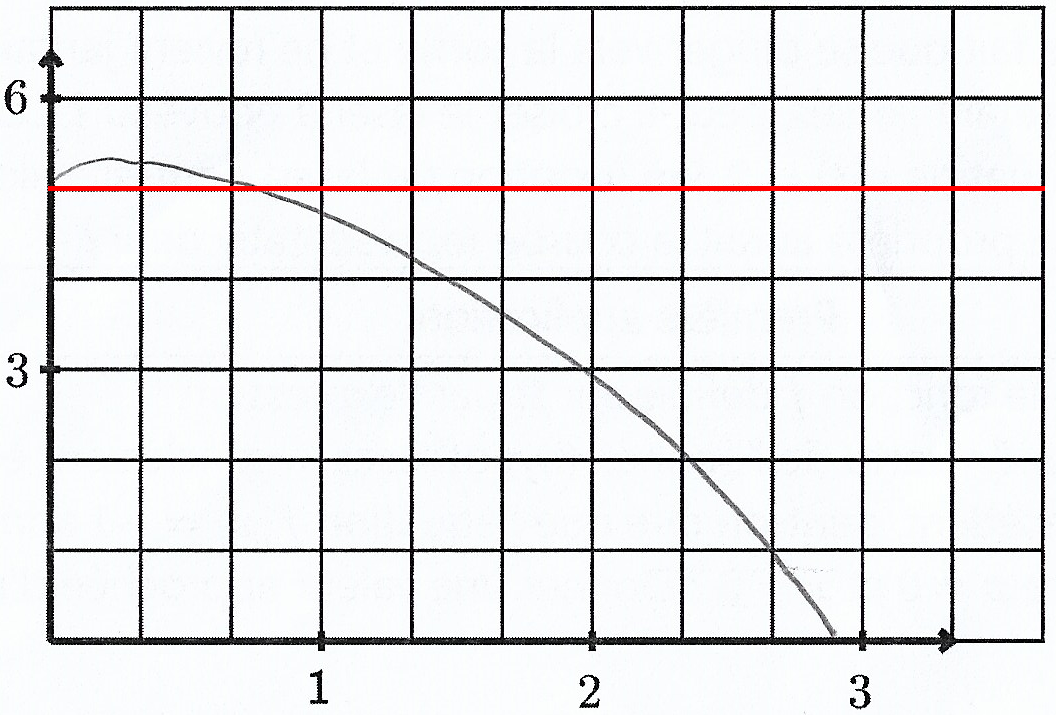
\includegraphics[scale=0.2]{TVI illus}
			\end{subfigure} }
			\hspace{20pt}
		 \scalebox{1}{ \begin{subfigure}[b!]{.5\textwidth}
				Question :
				\textit{L'équation $v(t)=5$ admet-elle une solution sur l'intervalle $[0;2]$ ?} \\
				Réponse :
				On sait que :
				\vspace{-3pt}
				\begin{itemize}
					\vspace{-3pt}
					\item \trou{$v$ est continue sur l'intervalle $[0;2]$ (à justifier),}
					\vspace{-3pt}
					\item \trou{$v(0)=5$ et $v(2)=3$ or $v(0) \geq 5 \geq v(2)$.}
				\end{itemize}
				\vspace{-3pt}
				Donc par le théorème des valeurs intermédiaires \trou{l'équation $v(t)=5$ admet \underline{au moins} une solution sur $[0;2]$.}
			\end{subfigure}
		}
		
	\end{figure}
	
\end{boiteExemple}

\vspace{-20pt}
\begin{boiteProposition}[title={Théorème des valeurs intermédiaires version monotone (admis)}]
On considère une fonction $f$ définie sur $[a;b]$ et un réel $k$. Si :
\vspace{-3pt}
\begin{itemize}
	\vspace{-3pt}
	\item \trou{$f$ est continue sur $[a;b]$ et \underline{strictement croissante} ou \underline{strictement décroissante},}
	\vspace{-3pt}
	\item \trou{$k$ est compris entre $f(a)$ et $f(b)$,}
\end{itemize}
\vspace{-3pt}
alors \trou{il existe \underline{un unique} $c \in [a;b]$ tel que $f(c)=k$. Autrement dit l'équation $f(x)=k$ admet une \underline{unique} solution : $x=c$.}
\end{boiteProposition}
\vspace{-10pt}
\begin{boiteExemple}[title={Exemples}]
	
	\vspace{-20pt}
	\begin{figure}[H]
		
		\centering
		\scalebox{1}{
			\begin{subfigure}[b!]{.4\textwidth}
				\centering
				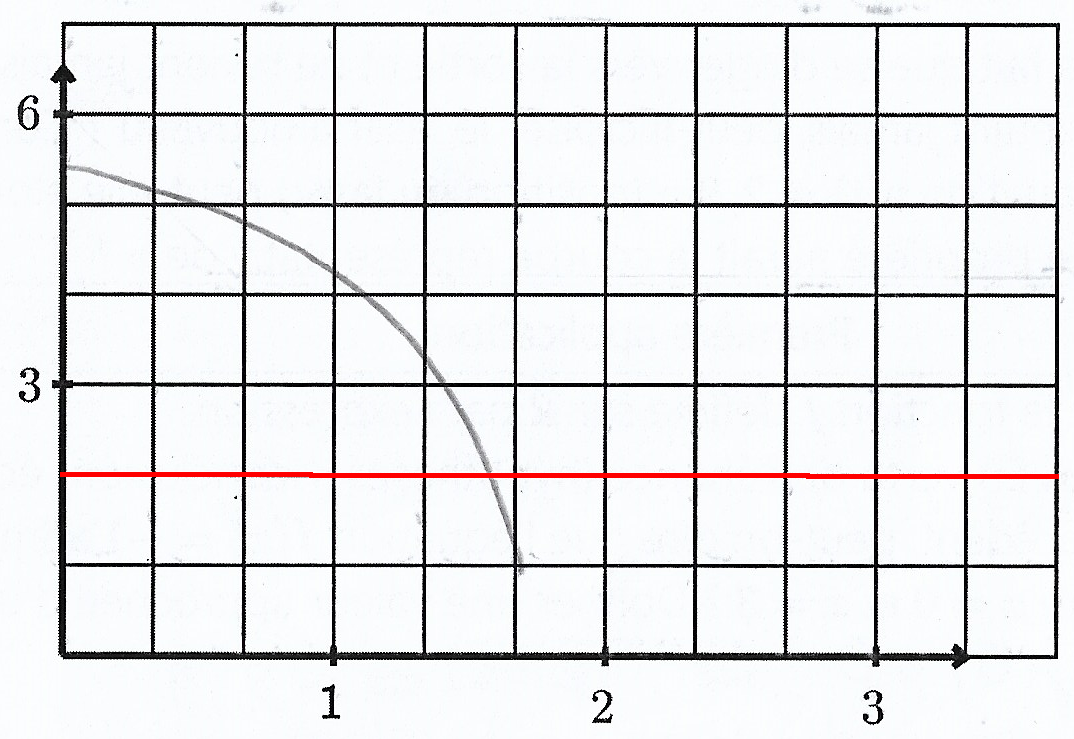
\includegraphics[scale=0.2]{TVI m illus}
				 
			\end{subfigure} }
			\hspace{20pt}
		 \scalebox{1}{ \begin{subfigure}[b!]{.5\textwidth}
				Question :
				\textit{L'équation $v(t)=2$ admet-elle une solution sur l'intervalle $[0;1,66]$ ?} \\
				Réponse :
				On sait que :
				\vspace{-3pt}
				\begin{itemize}
					\vspace{-3pt}
					\item \trou{$v$ est continue sur l'intervalle $[0;1,66]$ et \underline{strictement décroissante} (à justifier),}
					\vspace{-3pt}
					\item \trou{$v(0)=5,5$ et $v(1,66)=1$ donc $v(0) \geq 2 \geq v(1,66)$.}
				\end{itemize}
				\vspace{-3pt}
				Donc par le théorème des valeurs intermédiaires (version monotone) \trou{l'équation $v(t)=2$ admet une \underline{unique} une solution sur $[0;1,66]$.}
			\end{subfigure}
		}
		
	\end{figure}
	
\end{boiteExemple}

\end{document}